\documentclass[12pt]{article}
\usepackage[utf8]{inputenc}
\usepackage[a4paper, total={6in, 8in}, margin=1in]{geometry}
\usepackage{titlesec}
\usepackage[backend=biber, style=ieee]{biblatex}
\usepackage{graphicx}
\usepackage{amsmath}
\usepackage{amssymb}
\usepackage{amstext}
\usepackage{array}
\usepackage{xcolor}

\newcolumntype{L}{>{$}l<{$}}  % Math mode table
\newcolumntype{R}{>{$}r<{$}}  % Math mode table
\newcolumntype{C}{>{$}c<{$}}  % Math mode table

\addbibresource{main.bib}

\titleformat{\section}
  {\normalfont\fontsize{14}{15}\bfseries}{\thesection}{1em}{}

\titleformat{\subsection}
  {\normalfont\fontsize{12}{15}\bfseries}{\thesubsection}{1em}{}

\title{AES 561 Homework 4}
 \author{Mitchell Dodson}
\date{March 23, 2023}

\begin{document}

\maketitle

\section{Satellite Image Analysis}

\subsection{Brightness histograms and equalization}

\begin{figure}[h!]
    \centering
    \includegraphics[width=.48\linewidth]{figures/p1/mod_histograms.png}
    \includegraphics[width=.48\linewidth]{figures/p1/mod_cumulative.png}
    \includegraphics[width=.48\linewidth]{figures/p1/mod_histograms_correct.png}
    \caption{Brightness histograms, cumulative histograms, and discretized histogram-normalized distributions of MODIS bands M15, M11, M10, M05, M04, and M03.}
    \label{p1_histograms}
\end{figure}

\clearpage

\subsection{Image enhancement with histogram equalization}

\begin{figure}[h!]
    \centering
    \includegraphics[width=.49\linewidth]{figures/p2/naturalcolor_original.png}
    \includegraphics[width=.49\linewidth]{figures/p2/naturalcolor_histnorm.png}
    \caption{Original MODIS natural color RGB (bands I03, I02, and I01), and histogram-enhanced RGB, both normalized.}
    \label{p2_enhanced}
\end{figure}

\begin{figure}[h!]
    \centering
    \includegraphics[width=.48\linewidth]{figures/p2/img_histograms.png}
    \includegraphics[width=.48\linewidth]{figures/p2/img_histograms_correct.png}
    \caption{Original and histogram-corrected brightness frequency distribution hisograms for each MODIS imagery band used in the naturalcolor image.}
    \label{p2_histograms}
\end{figure}

\begin{figure}[h!]
    \centering
    \includegraphics[width=.48\linewidth]{figures/p2/truecolor_contrast.png}
    \includegraphics[width=.48\linewidth]{figures/p2/img_histograms_contrast.png}
    \caption{Natural color RGB enhanced with the saturating linear contrast method, and its brightness frequency histogram.}
    \label{p2_histograms}
\end{figure}

\clearpage

\subsection{Classification candidate selection}

\begin{figure}[h!]
    \centering
    \includegraphics[width=.50\linewidth]{figures/p4/region_indicator.png}
    \includegraphics[width=.48\linewidth]{figures/p4/pixel_area_ratio_bordered.png}
    \caption{These images give context on the region I selected. The first image indicates my region's extent in the West US with the blue rectangle, and the second shows the pixelwise area distortion in my domain, with white representing greater distortion. The Suomi-NPP MODIS granule I retrieved for my region was captured on July 12, 2016 at 2006z. The center of my image is slightly East of the nadir point, so the East edge is subject to the greatest panoramic distortion. The approximate surface area of my region is $200,691.53\,km^2$.}
    \label{p3_region}
\end{figure}

\begin{figure}[h!]
    \centering
    \includegraphics[width=.7\linewidth]{figures/p3/selections.png}
    \caption{Pixel selections for each class used as training inputs. Cloud samples are shown in teal, crops samples are shown in bright green, mountain vegetation samples are shown in dark green, water samples are shown in blue, grassland samples are shown in yellow, and red sand/clay samples are shown in orange.}
    \label{p3_pixels}
\end{figure}

\begin{figure}[h!]
    \centering
    \includegraphics[width=.48\linewidth]{figures/p3/selectionRGB_M05-M04-M03_tcEQ.png}
    \includegraphics[width=.48\linewidth]{figures/p3/selectionRGB_M15-NDVI-NDSI_custom.png}

    \vspace{.2em}
    \includegraphics[width=.48\linewidth]{figures/p3/selectionRGB_M09-M05-M10_dcp.png}
    \caption{MODIS RGBs used for pixel class selection.}
    \label{p3_selection_rgbs}
\end{figure}

Figure \ref{p3_selection_rgbs} displays the RGBs I used to pick samples for pixel classes, the first image is an equalized truecolor image with bands M05, M04, and M03, the second image is a gamma-enhanced day-cloud phase RGB adaptation of the GOES ABI recipe using bands M09, M05, and M10, and the third image is a histogram-enhanced custom recipe of band M15, M07-M05 NDVI, and M10-M04 NDSI, which I created in order to easily distinguish clouds and multiple surface types. Band M15, which has a peak wavelength near $10.8\mu m$, is sensitive to the emissivity properties of surfaces, which makes it easy to distinguish red clay from arid grassland, NDVI makes vegetation very visible, and NDSI incidentally distinguishes exposed and rocky areas from vegetation and grassland better than the truecolor.

\begin{figure}
    \centering
    \begin{tabular}{R | C C | C C | C C | C C | C C}
        & \multicolumn{2}{c|}{M15} & \multicolumn{2}{c|}{M14} & \multicolumn{2}{c|}{M12} & \multicolumn{2}{c|}{M10} & \multicolumn{2}{c}{M09} \\
        \textnormal{Category} & \mu_1 & \sigma_1 & \mu_2 & \sigma_2 & \mu_3 & \sigma_3 & \mu_4 & \sigma_4 & \mu_5 & \sigma_5 \\
        \hline
        \textnormal{Cloud} & 5.545 & 1.539  & 4.784 & 1.686  & 0.913 & 0.173  & 0.552 & 0.151  & 0.215 & 0.098 \\
        \textnormal{Water} & 10.220 & 1.352  & 9.697 & 1.429  & 0.803 & 0.268  & 0.147 & 0.078  & 0.001 & 0.001 \\
        \textnormal{Mtn Veg} & 9.683 & 0.510  & 9.242 & 0.584  & 0.519 & 0.098  & 0.155 & 0.026  & 0.003 & 0.001 \\
        \textnormal{Clay} & 13.186 & 0.415  & 12.698 & 0.540  & 1.479 & 0.150  & 0.358 & 0.063  & 0.003 & 0.001 \\
        \textnormal{Grassland} & 13.389 & 0.511  & 13.171 & 0.502  & 1.500 & 0.156  & 0.372 & 0.061  & 0.003 & 0.002 \\
        \textnormal{Crops} & 10.575 & 0.685  & 10.188 & 0.769  & 0.719 & 0.161  & 0.220 & 0.032  & 0.002 & 0.001 \\
    \end{tabular}

    \vspace{1em}

    \begin{tabular}{R | C C | C C | C C | C C}
        & \multicolumn{2}{c|}{M07} & \multicolumn{2}{c|}{M05} & \multicolumn{2}{c|}{M04} & \multicolumn{2}{c}{M03} \\
        \textnormal{Category} & \mu_6 & \sigma_6 & \mu_7 & \sigma_7 & \mu_8 & \sigma_8 & \mu_9 & \sigma_9 \\
        \hline
        \textnormal{Cloud} & 0.676 & 0.215  & 0.611 & 0.227  & 0.581 & 0.215  & 0.590 & 0.220 \\
        \textnormal{Water} & 0.141 & 0.065  & 0.118 & 0.041  & 0.117 & 0.024  & 0.118 & 0.019 \\
        \textnormal{Mtn Veg} & 0.269 & 0.046  & 0.049 & 0.010  & 0.071 & 0.008  & 0.068 & 0.007 \\
        \textnormal{Clay} & 0.291 & 0.052  & 0.204 & 0.045  & 0.128 & 0.018  & 0.117 & 0.012 \\
        \textnormal{Grassland} & 0.301 & 0.031  & 0.231 & 0.038  & 0.186 & 0.027  & 0.164 & 0.019 \\
        \textnormal{Crops} & 0.411 & 0.065  & 0.091 & 0.024  & 0.107 & 0.012  & 0.094 & 0.012 \\
    \end{tabular}
    \caption{Means and standard deviations of pixels selected as samples for each surface category.}
    \label{p3_stats}
\end{figure}

\clearpage

\subsection{Minimum-distance classification}

\begin{figure}[h!]
    \centering
    \includegraphics[width=.8\linewidth]{figures/p4/mdc_4+5.png}
    \caption{Minimum-distance classification of my region using all bands listed in Fig \ref{p3_stats}.}
    \label{p4_mdc}
\end{figure}


\begin{figure}[h!]
    \centering
    \begin{tabular}{r | C | C C | C C | C C | C C }
        \multicolumn{2}{c}{} & \multicolumn{2}{c|}{M15} & \multicolumn{2}{c|}{M14} & \multicolumn{2}{c|}{M12} & \multicolumn{2}{c}{M10} \\
        Category & \textnormal{Area ($km^2$)} & \mu_1 & \sigma_1 & \mu_2 & \sigma_2 & \mu_3 & \sigma_3 & \mu_4 & \sigma_4 \\
        \hline
        Cloud & 2,797 & 5.488 & 1.516  & 4.722 & 1.661  & 0.911 & 0.169  & 0.552 & 0.148  \\
        Water & 19,109 & 10.164 & 1.359  & 9.637 & 1.437  & 0.795 & 0.266  & 0.144 & 0.077  \\
        Mtn Veg  & 29,993 & 9.724 & 0.537  & 9.291 & 0.619  & 0.527 & 0.104  & 0.156 & 0.027  \\
        Clay & 81,778 & 13.189 & 0.429  & 12.706 & 0.550  & 1.478 & 0.153  & 0.354 & 0.063  \\
        Grassland & 31,163 & 13.369 & 0.517  & 13.154 & 0.514  & 1.490 & 0.159  & 0.372 & 0.059  \\
        Crops & 35,850 & 10.560 & 0.675  & 10.172 & 0.758  & 0.715 & 0.159  & 0.218 & 0.032  \\
    \end{tabular}

    \vspace{1em}

    \begin{tabular}{r | C C | C C | C C | C C | C C}
        & \multicolumn{2}{c|}{M09} & \multicolumn{2}{c|}{M07} & \multicolumn{2}{c|}{M05} & \multicolumn{2}{c|}{M04} & \multicolumn{2}{c}{M03} \\
        \textnormal{Category} & \mu_5 & \sigma_5 & \mu_6 & \sigma_6 & \mu_7 & \sigma_7 & \mu_8 & \sigma_8 & \mu_9 & \sigma_9 \\
        \hline
        Cloud & 0.218 & 0.098 & 0.411 & 0.065  & 0.091 & 0.023  & 0.107 & 0.012  & 0.094 & 0.012 \\
        Water & 0.001 & 0.001 & 0.299 & 0.031  & 0.228 & 0.040  & 0.184 & 0.028  & 0.162 & 0.019 \\
        Mtn veg & 0.003 & 0.001 & 0.289 & 0.051  & 0.203 & 0.044  & 0.127 & 0.018  & 0.116 & 0.012 \\
        Clay & 0.003 & 0.001 & 0.269 & 0.044  & 0.050 & 0.011  & 0.071 & 0.008  & 0.069 & 0.007 \\
        Grassland & 0.003 & 0.002 & 0.139 & 0.065  & 0.117 & 0.041  & 0.116 & 0.024  & 0.118 & 0.019 \\
        Crops & 0.002 & 0.001 & 0.682 & 0.214  & 0.619 & 0.226  & 0.588 & 0.214  & 0.598 & 0.219 \\
    \end{tabular}
    \caption{Area coverage}
    \label{p4_stats}
\end{figure}

\clearpage

\subsection{Maximum-likelihood classification}

\begin{figure}[h!]
    \centering
    \includegraphics[width=.7\linewidth]{figures/p5/heatmap_M10+M15.png}

    \vspace{.2em}
    \includegraphics[width=.48\linewidth]{figures/p5/band_M10.png}
    \includegraphics[width=.48\linewidth]{figures/p5/band_M15.png}
    \caption{Intensity heat map of bands M10 and M15, and greyscale images of band M10 and M15, respectively. Band M10 peaks at $1.61\mu m$, and band M15 peaks at $10.76\mu m$. I chose these bands because the nonlinear heatmap suggests that the similarities of some surface types are easier to isolate when the surfaces' properties differ between bands.}
    \label{p5_inputs}
\end{figure}

\begin{figure}[h!]
    \centering
    \includegraphics[width=.7\linewidth]{figures/p5/mlc_4+5_M10+M15.png}

    \vspace{.2em}
    \includegraphics[width=.7\linewidth]{figures/p5/mlc_4+5_M15+M14+M12+M10+M09+M07+M05+M04+M03.png}
    \caption{Maximum-likelihood classification of my region. The first image shows classes assigned using only bands M10 and M15, and the second image shows classes assigned using all 9 bands I selected. The 2-band version has high skill in distinguishing clouds and vegetation from other surface types, but misclassified snow on the mountain peaks as water, and misclassified much of the unvegetated ground. The all-band version had much higher skill, and closely emulated the surfaces I selected for my training samples.}
    \label{p5_mlc}
\end{figure}

\begin{figure}[h!]
    \centering
    \begin{tabular}{ r | C | C C | C C }
        \multicolumn{2}{c|}{} & \multicolumn{2}{c|}{M10} & \multicolumn{2}{c}{M15} \\
        Category & \textnormal{Area ($km^2$)} & \mu_1 & \sigma_1 & \mu_2 & \sigma_2 \\
        \hline
        Cloud & 4,860 & 0.468 & 0.139  & 6.783 & 1.569 \\
        Water & 818 & 0.103 & 0.023  & 9.278 & 0.389 \\
        Mtn Veg & 34,785 & 0.183 & 0.037  & 10.509 & 0.917 \\
        Clay & 83,785 & 0.288 & 0.039  & 12.586 & 0.683 \\
        Grassland & 43,843 & 0.391 & 0.037  & 13.233 & 0.447 \\
        Crops & 32,601 & 0.217 & 0.025  & 10.460 & 0.532 \\
    \end{tabular}
    \caption{Bands M10 and M15 maximum-likelihood mean and standard deviation for each category, and each category's area coverage.}
    \label{p5_2band_stats}
\end{figure}

\begin{figure}[h!]
    \centering
    \begin{tabular}{r | C | C C | C C | C C | C C }
        \multicolumn{2}{c|}{} & \multicolumn{2}{c|}{M15} & \multicolumn{2}{c|}{M14} & \multicolumn{2}{c|}{M12} & \multicolumn{2}{c}{M10} \\
        Category & \textnormal{Area ($km^2$)} & \mu_1 & \sigma_1 & \mu_2 & \sigma_2 & \mu_3 & \sigma_3 & \mu_4 & \sigma_4 \\
        \hline
        Cloud & 8,397 & 8.204 & 2.130  & 7.705 & 2.334  & 0.896 & 0.191  & 0.378 & 0.158 \\
        Water & 246 & 9.533 & 0.907  & 8.986 & 0.999  & 0.669 & 0.200  & 0.109 & 0.053 \\
        Mtn Veg & 52,797 & 10.512 & 0.831  & 10.195 & 0.961  & 0.699 & 0.169  & 0.195 & 0.037 \\
        Clay & 52,412 & 12.445 & 0.842  & 12.144 & 0.879  & 1.208 & 0.243  & 0.290 & 0.068 \\
        Grassland & 77,052 & 12.897 & 0.816  & 12.707 & 0.899  & 1.331 & 0.216  & 0.339 & 0.056 \\
        Crops & 9,785 & 11.194 & 0.698  & 10.892 & 0.806  & 0.848 & 0.163  & 0.234 & 0.032 \\
    \end{tabular}

    \vspace{1em}

    \begin{tabular}{r | C C | C C | C C | C C | C C}
        & \multicolumn{2}{c|}{M09} & \multicolumn{2}{c|}{M07} & \multicolumn{2}{c|}{M05} & \multicolumn{2}{c|}{M04} & \multicolumn{2}{c}{M03} \\
        \textnormal{Category} & \mu_5 & \sigma_5 & \mu_6 & \sigma_6 & \mu_7 & \sigma_7 & \mu_8 & \sigma_8 & \mu_9 & \sigma_9 \\
        \hline
        Cloud & 0.096 & 0.087  & 0.405 & 0.194  & 0.310 & 0.206  & 0.296 & 0.193  & 0.299 & 0.198 \\
        Water & 0.001 & 0.000  & 0.108 & 0.046  & 0.096 & 0.031  & 0.107 & 0.027  & 0.111 & 0.022 \\
        Mtn Veg & 0.004 & 0.002  & 0.256 & 0.041  & 0.070 & 0.017  & 0.083 & 0.011  & 0.079 & 0.010 \\
        Clay & 0.003 & 0.001  & 0.251 & 0.047  & 0.151 & 0.051  & 0.117 & 0.021  & 0.110 & 0.016 \\
        Grassland & 0.003 & 0.002  & 0.276 & 0.031  & 0.186 & 0.042  & 0.155 & 0.027  & 0.141 & 0.019 \\
        Crops & 0.002 & 0.001  & 0.317 & 0.061  & 0.101 & 0.021  & 0.108 & 0.011  & 0.100 & 0.010 \\
    \end{tabular}
    \caption{All-band maximum-likelihood mean and standard deviation of each band for each category, and each category's area coverage.}
    \label{p5_allband_stats}
\end{figure}

\clearpage

\subsection{K-means classification}

\begin{figure}[h!]
    \centering
    \includegraphics[width=.48\linewidth]{figures/p6/k-means_M10+M15_4cat.png}
    \includegraphics[width=.48\linewidth]{figures/p6/k-means_M10+M15_5cat.png}
    \includegraphics[width=.48\linewidth]{figures/p6/k-means_M10+M15_6cat.png}
    \caption{K-means classification using bands M10 and M15. Images are initialized with 4, 5, and 6 categories, respectively.}
    \label{p6_456_classes}
\end{figure}

\begin{figure}[h!]
    \centering
    \includegraphics[width=.7\linewidth]{figures/p6/k-means_M10+M15_5cat_noborder.png}
    \caption{5-category k-means classification with bands M10 and M15. }
    \label{p6_noborder}
\end{figure}

\begin{figure}[h!]
    \centering
    \begin{tabular}{r | C | C C | C C |}
        Class & \textnormal{Count} & \textnormal{M10 $\mu$} & \textnormal{M10 $\sigma$} & \textnormal{M15 $\mu$} & \textnormal{M15 $\sigma$} \\
        \hline
        Class 1 & 181779 & 0.267 & 0.039 & 1.306 & 0.174 \\
        Class 2 & 95648 & 0.261 & 0.048 & 0.799 & 0.134 \\
        Class 3 & 34619 & 0.268 & 0.067 & 0.565 & 0.143 \\
        Class 4 & 11051 & 0.289 & 0.033 & 1.651 & 0.067 \\
        Class 5 & 4583 & 0.612 & 0.172 & 0.933 & 0.134 \\
    \end{tabular}
    \caption{Pixel counts, mean, and standard deviation of each pixel class identified by K-means classification with bands M10 and M15.}
\end{figure}

\clearpage

\subsection{Principle component analysis}

%\begin{figure}
%    \centering
%    \begin{equation}\nonumber
%        \begin{pmatrix}
%            2.3843 & 2.5338 & 0.4513 & 0.0596 & -0.0204 & -0.0259 & 0.0245 & -0.0050 & -0.0125 \\
%            2.5338 & 2.7256 & 0.4703 & 0.0585 & -0.0218 & -0.0313 & 0.0211 & -0.0076 & -0.0151 \\
%            0.4513 & 0.4703 & 0.1151 & 0.0233 & -0.0006 & 0.0027 & 0.0175 & 0.0089 & 0.0072 \\
%            0.0596 & 0.0585 & 0.0233 & 0.0076 & 0.0008 & 0.0033 & 0.0064 & 0.0043 & 0.0039 \\
%            -0.0204 & -0.0218 & -0.0006 & 0.0008 & 0.0006 & 0.0011 & 0.0013 & 0.0013 & 0.0013 \\
%            -0.0259 & -0.0313 & 0.0027 & 0.0033 & 0.0011 & 0.0041 & 0.0036 & 0.0031 & 0.0030 \\
%            0.0245 & 0.0211 & 0.0175 & 0.0064 & 0.0013 & 0.0036 & 0.0065 & 0.0048 & 0.0045 \\
%            -0.0050 & -0.0076 & 0.0089 & 0.0043 & 0.0013 & 0.0031 & 0.0048 & 0.0039 & 0.0038 \\
%            -0.0125 & -0.0151 & 0.0072 & 0.0039 & 0.0013 & 0.0030 & 0.0045 & 0.0038 & 0.0038 \\
%        \end{pmatrix}
%    \end{equation}
%
%    \begin{tabular}{ C | C C C C C C C C C}
%        \lambda & \vec{v}_1 & \vec{v}_2  & \vec{v}_3  & \vec{v}_4  & \vec{v}_5  & \vec{v}_6  & \vec{v}_7  & \vec{v}_8  & \vec{v}_9 \\
%        \hline
%        0.0001 & 0.006 & -0.331 & -0.087 & -0.157 & 0.414 & -0.062 & 0.092 & 0.648 & -0.502 \\
%        0.0001 & -0.003 & -0.237 & -0.172 & -0.151 & 0.453 & -0.186 & 0.661 & -0.382 & 0.259 \\
%        0.0001 & -0.001 & -0.248 & -0.151 & -0.211 & 0.436 & -0.128 & -0.716 & -0.098 & 0.373 \\
%        0.0006 & -0.007 & -0.209 & -0.034 & -0.695 & -0.544 & -0.415 & 0.027 & 0.029 & 0.007 \\
%        0.0008 & -0.005 & -0.076 & -0.083 & 0.006 & 0.056 & -0.109 & -0.197 & -0.632 & -0.729 \\
%        0.0022 & 0.016 & -0.316 & -0.057 & -0.351 & -0.091 & 0.865 & 0.029 & -0.120 & -0.003 \\
%        0.0131 & 0.127 & -0.740 & -0.133 & 0.541 & -0.326 & -0.095 & -0.012 & 0.001 & 0.086 \\
%        0.0542 & 0.724 & 0.244 & -0.639 & -0.020 & -0.055 & 0.026 & 0.001 & 0.053 & -0.013 \\
%        5.180 & 0.677 & -0.115 & 0.708 & -0.079 & 0.116 & -0.037 & -0.000 & -0.068 & -0.001 \\
%    \end{tabular}
%    \caption{Covariance matrix and eigenvalues ($\lambda$) and normalized eigenvector components ($\vec{v})$ used for principle component analysis of my region.}
%\end{figure}

\begin{figure}[h!]
    \begin{center}
    $
    \begin{pmatrix}
        0.0065 & 0.0036 & 0.0245 \\
        0.0036 & 0.0041 & -0.0259 \\
        0.0245 & -0.0259 & 2.3843 \\
    \end{pmatrix}
    $
    \begin{tabular}{ C | C | C C C }
        & \lambda & \vec{v}_1 & \vec{v}_2 & \vec{v}_3 \\
        \hline
        PC1 & 2.3848 & -0.0103 & -0.8063 & 0.5915 \\
        PC2 & 0.0091 & 0.0109 & -0.5915 & -0.8062 \\
        PC3 & 0.0010 & -0.9999 & 0.0019 & -0.0148 \\
    \end{tabular}
    \end{center}
    \caption{Covariance matrix, eigenvalues ($\lambda$), and normalized eigenvector components ($\vec{v}$) used for principle component analysis of my region.}
    \label{p7_cov_ev}
\end{figure}


\begin{figure}[h!]
    \centering
    \includegraphics[width=.6\linewidth]{figures/p7/pca_4+6+8_eq.png}

    \vspace{.2em}
    \includegraphics[width=.4\linewidth]{figures/p7/pca_0+3+5_eq.png}
    \includegraphics[width=.4\linewidth]{figures/p7/region_M05+M07+M15.png}
    \caption{Principle component analysis results. The fist image was generated using only bands M05, M07, and M15, and the second shows 3 of the 9 components found when all 9 bands were used for PCA. The third image is a normalized RGB of bands M05, M07, and M15. Compared to the original composite, the 3-band image is good at resolving clouds and multiple surface types, but still doesn't easily isolate water or vegetation types, and the all-band components I chose are skillful at distinguishing vegetation types and surface texture, but fails to clearly distinguish clouds from mountain vegetation. Judging by the color distribution of the 3-band image, the red component appears to scale positively with highly vegetated surfaces and negatively with clouds, the green band correlates with cloud cover and vegetation, and the blue band correlates with bare ground.}
    \label{p7_results}
\end{figure}

\clearpage

\subsection{Edge detection}

\begin{figure}[h!]
    \centering
    \includegraphics[width=.48\linewidth]{figures/p8/aster_vertical.png}
    \includegraphics[width=.48\linewidth]{figures/p8/aster_horizontal.png}

    \vspace{.2em}
    \includegraphics[width=.48\linewidth]{figures/p8/aster_diagonal1.png}
    \includegraphics[width=.48\linewidth]{figures/p8/aster_diagonal2.png}
    \caption{ASTER image after application of vertical, horizontal, forward diagonal, and back diagonal filters, respectively. Fine structures are much easier to identify when they run parallel to an edge filter's kernel. For example, the vertical lines of the harbor are easier to resolve in the vertically-filter image, and the San Mateo-Hayward Bridge is easiest to identify in the images filtered with horizontal and forward-diagonal kernels.}
    \label{p8_edgesteps}
\end{figure}

\begin{figure}[h!]
    \centering
    \includegraphics[width=.6\linewidth]{figures/p8/aster_original.png}

    \vspace{.2em}
    \includegraphics[width=.48\linewidth]{figures/p8/aster_sequential.png}
    \includegraphics[width=.48\linewidth]{figures/p8/aster_multi.png}

    \caption{Original ASTER image, edge detection using consecutive application of filters, histogram-equalized edge detection using each filter applied independently, then combined with euclidean distance in the same manner as the Sobel operator. Both edge detection methods appear to be effective, but even after histogram equalization the image generated with sequentially-applied filters appears noisier and more difficult to resolve than the euclidean distance scheme.}
    \label{p8_edgeresults}
\end{figure}

\clearpage

\subsection{Roberts and Sobel operators}

\begin{figure}[h!]
    \centering
    \includegraphics[width=.6\linewidth]{figures/p9/aster_roberts.png}

    \vspace{.2em}
    \includegraphics[width=.6\linewidth]{figures/p9/aster_sobel.png}

    \caption{ASTER image after applications of the Roberts and the Sobel operators, respectively. The results for each method are similar overall, but the Sobel operator resolves edges more finely, and doesn't generate as much noise in areas with features that are too small to be reasonably considered edges.}
    \label{p9_rob_sob}
\end{figure}

\clearpage

\subsection{Landsat MSS cloud and water-masked NDVI}

\begin{figure}[h!]
    \centering
    \includegraphics[width=.48\linewidth]{figures/p10/ndvi_masked_skparams.png}
    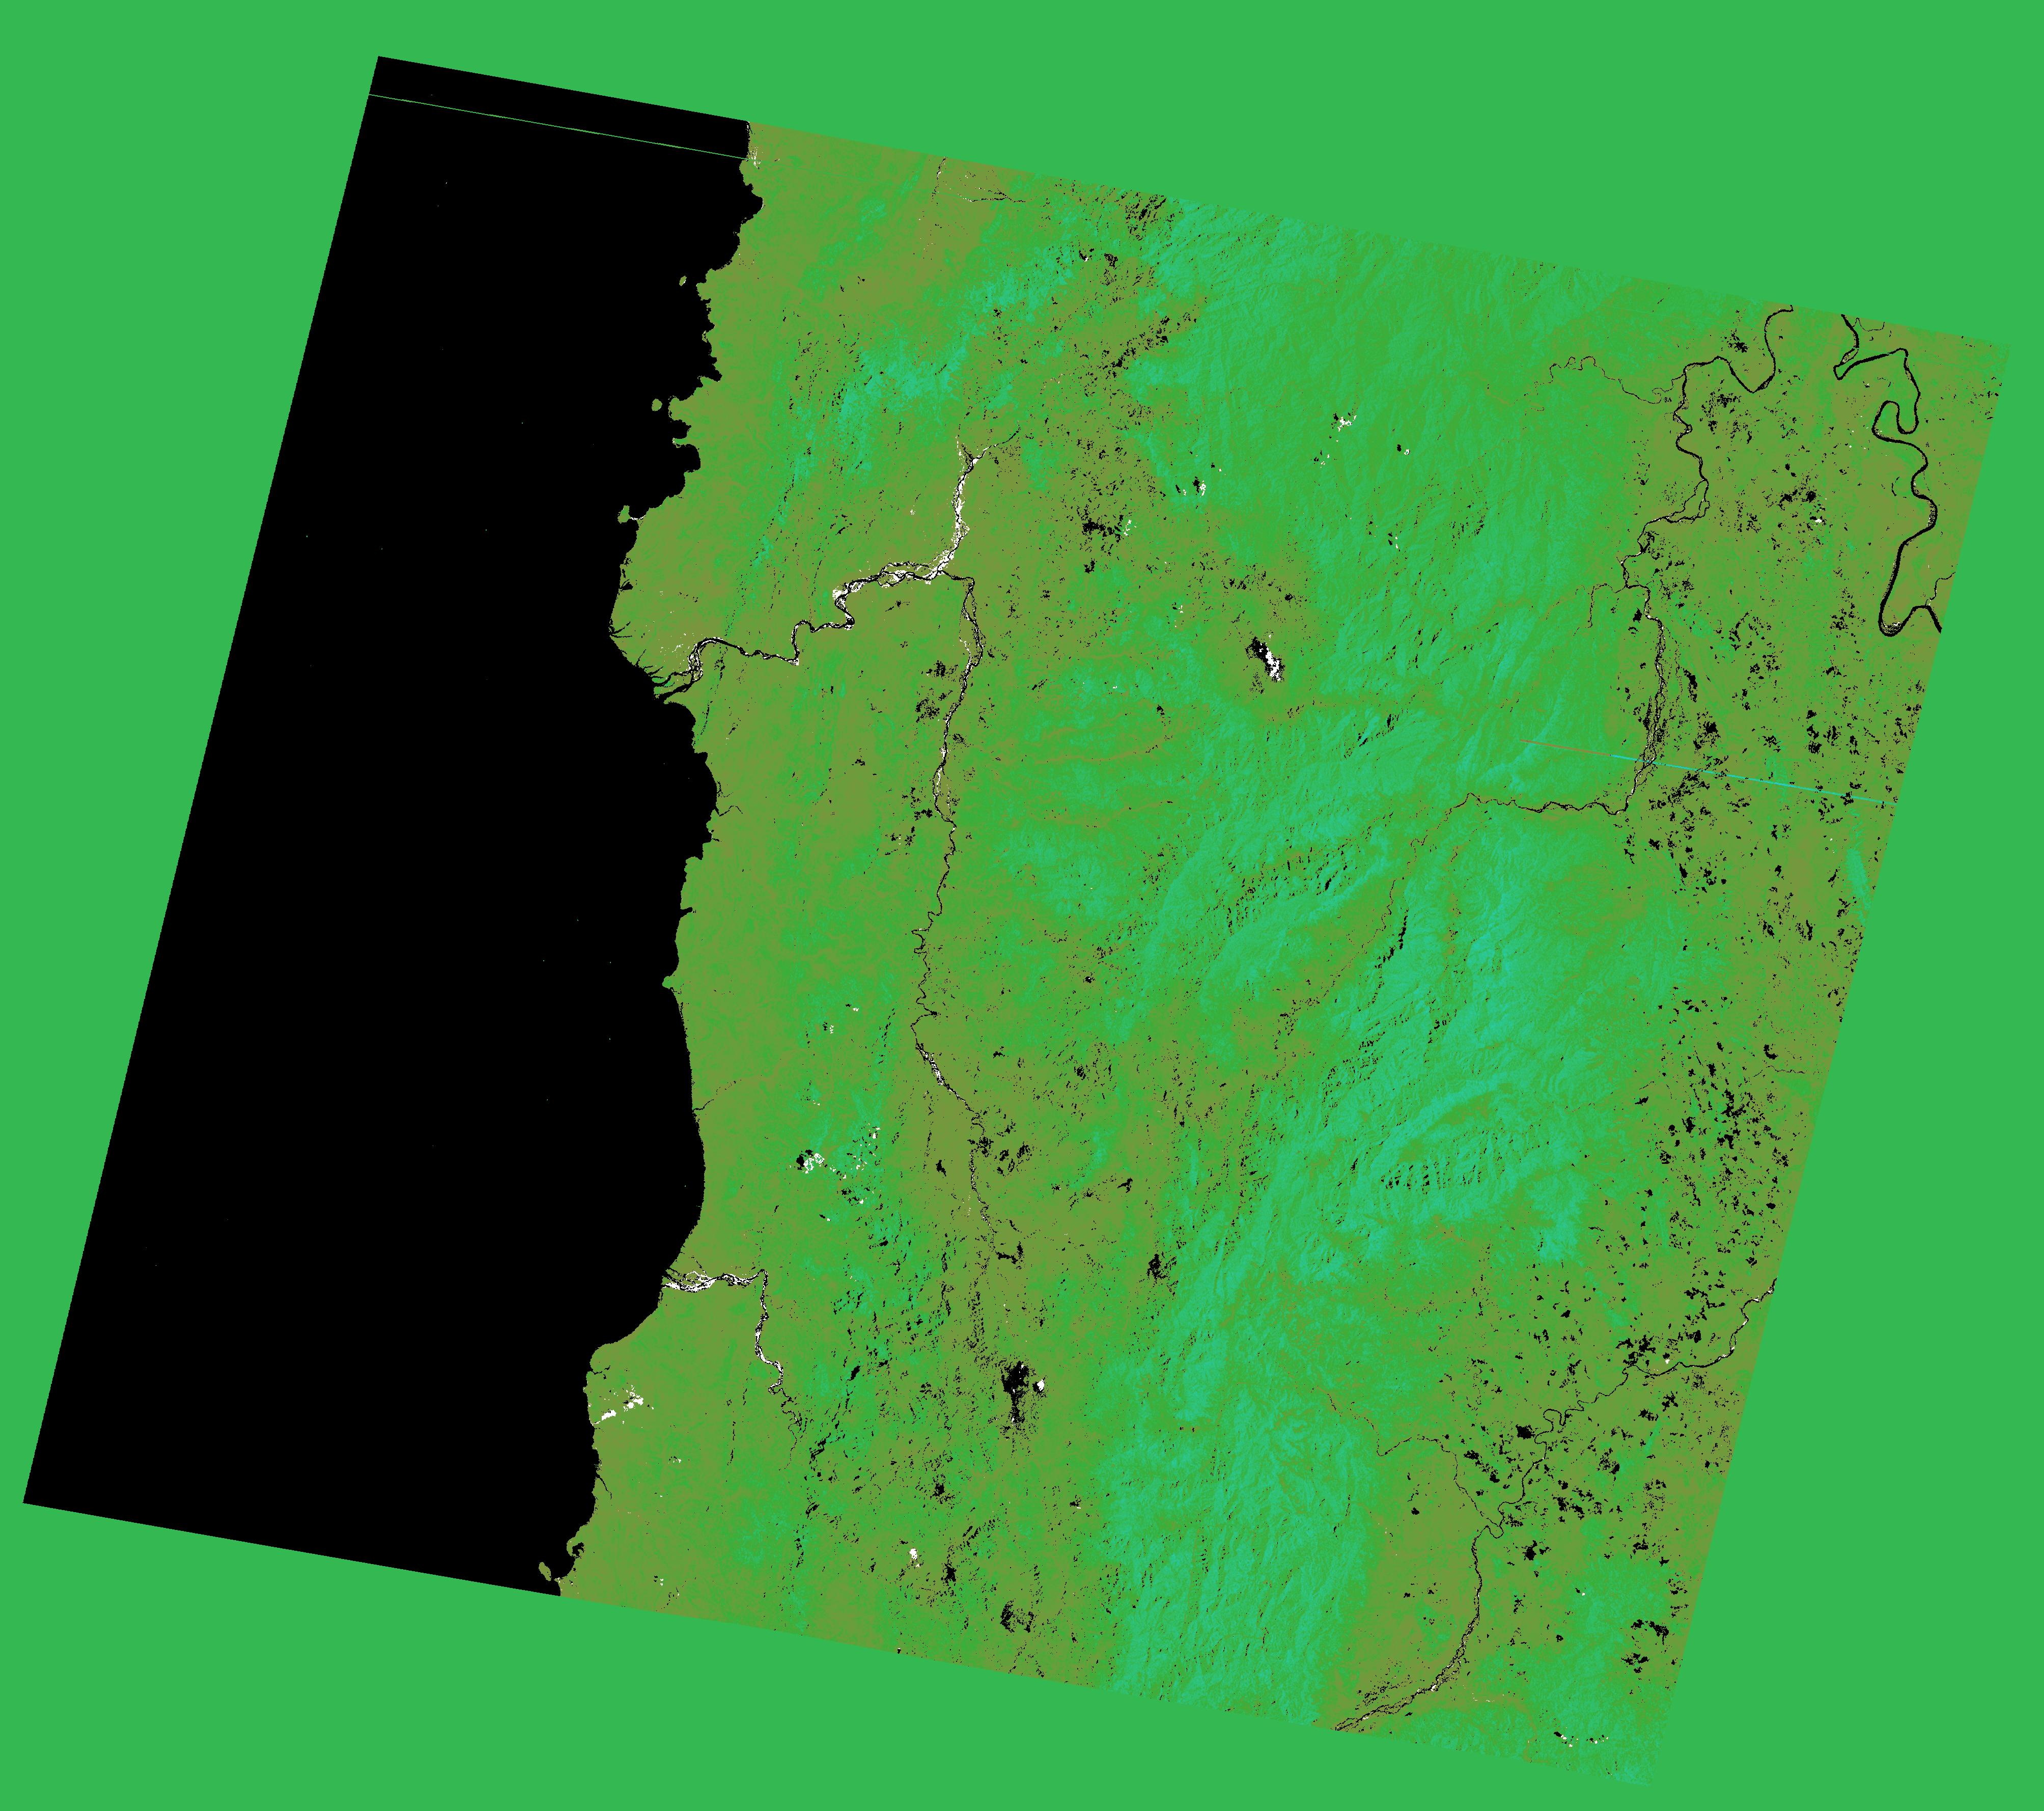
\includegraphics[width=.48\linewidth]{figures/p10/ndvi_masked_myparams.png}

    \vspace{.2em}
    \includegraphics[width=.48\linewidth]{figures/p10/cbar.png}
    \caption{Normalized NDVIs with clouds masked as white, and water masked as black. In both images, water is masked using the NDWI recipe (GREEN-NIR)/(GREEN+NIR) with Landsat MSS bands 1 ($0.5-0.6\mu m$) and 3 ($0.7-0.8\mu m$). The first image applies the Saunders \& Kriebel method as closely as possible, substituting AVHRR band 1 ($.62\mu m$) for Landsat band 1, and AVHRR band 2 ($.8\mu m$) for Landsat band 4 ($0.8-1.1\mu m$). The second image is an adaptation of the S\&K method using custom thresholds. The colorbar at the bottom is a rendering of the 256 brightness bins used in generating the NDVI RGB.}
    \label{p9_landsat}
\end{figure}

\begin{figure}[h!]
    \centering
    \begin{tabular}{ c c c c }
        Maximum & Minimum & Mean & Std. Dev. \\
        \hline
        0.7125 & 0.0570 & 0.5041 & 0.0079 \\
    \end{tabular}
    \caption{Statistics for masked NDVI values.}
    \label{p9_stats}
\end{figure}

Figure \ref{p9_landsat} displays my results as an HSV-mapped RGB with gamma enhancement, and Figure \ref{p9_stats} shows statistics on the NDVI values that weren't masked as clouds or water. The granule I used was captured by Landsat 3 over the Banaue Rice Terraces on Luzon island in the Phillipines on March 11, 1979. The rice paddy terraces are positioned East of the Lagban river, in the region with the highest NDVI values. In order to mask water in my image, I simply set a lower-bound threshold of $.39$ on the NDWI recipe specified in Figure \ref{p9_landsat}. Since the MSS instrument on Landsat 3 isn't equipped with any thermal IR bands (except for the one that failed soon after launch), I only performed tests 3 and 4 of the Saunders \& Kriebel method. Tests 3 and 4 stipulate that a cloud candidate must have a RED band reflectance greater than $15\%$, and a NIR to RED band ratio less than $1.6$. These thresholds weren't restrictive enough to be effective on my image, probably due to the additional atmospheric absorption in the NIR region covered by MSS band 4. When I increased test 1's threshold to a $38\%$ lower bound for the RED band and decreased test 2's NIR/RED ratio threshold to a $.9$ lower bound, the test successfully masked the few cumulus clouds in my image, as well as some valley fog on the Lagben river.

\clearpage

\subsection{Amazon fire detection}

\begin{figure}[h!]
    \centering
    \includegraphics[width=.99\linewidth]{figures/p11/fire_mosaic_labeled.png}
    \caption{Mosaic of the progression of the field fire I selected, which burned September 3-5, 2018. The \textsc{x} marks the pixel closest to $60^\circ W$, $10^\circ S$. I specifically focus on the image captured by Aqua on September 4 at 1715z. This granule was acquired only 3 minutes prior to the JPSS-1 VIIRS granule shown in the top right.}
    \label{p11_mosaic}
\end{figure}

\begin{figure}[h!]
    \centering
    \includegraphics[width=.32\linewidth]{figures/p11/amazon_fireRGB_IRdiff+LWIR+VIS.png}
    \includegraphics[width=.32\linewidth]{figures/p11/amazon_fc_cand.png}
    \includegraphics[width=.32\linewidth]{figures/p11/amazon_fc_fires.png}
    \caption{My custom-enhanced fire RGB, pixels identified as fire candidates by the Flasse \& Ceccato (F\&C) method, and fires confirmed by F\&C. 5,982 pixels were positively identified as fires with the standard thresholds.}
    \label{p11_fc}
\end{figure}

\begin{figure}[h!]
    \centering
    \includegraphics[width=.45\linewidth]{figures/p11/amazon_my_candidates.png}
    \includegraphics[width=.45\linewidth]{figures/p11/amazon_my_fires.png}
    \caption{Pixels identified as fire candidates using custom thresholds, and subsequent pixels identified as fires with the F\&C confirmation methodology. When selecting pixel candidates, I decreased the SWIR lower bound from $314K$ to $311K$, decreased the SWIR-LWIR difference threshold to $8K$, decreased the upper bound of NIR reflectivity to $10 \%$, and set a new lower bound of $280 K$ on the LWIR threshold. I chose these values to better approximate the locations of the relatively isolated red pixels in my fire RGB, as the standard F\&C method demonstrated in Figure \ref{p11_fc} seemed to classify fires far too generously. The only significant differences between the pixel candidates my threshold selected and the pixels confirmed to be fires are that some groupings of candidate pixels over the low-lying clouds in the bottom right were disqualified as fires by the F\&C algorithm. I believe these changes were necessary because I substituted AVHRR band 2 ($.725-1.0\mu m$) for the average reflectance of MODIS bands 4, 3, and 1 ($.459-.670\mu m$ in total) since no NIR bands were available in the L1b granule I used. The $.8-1\mu m$ edge of the blackbody radiance curve for a $1000K$ fire is small, but much greater than in the visible range, and NIR wavelengths are attenuated less by Rayleigh scattering than in the visible spectrum. Either or both of these factors may have contributed to decreasing observed radiance in the MODIS visible bands compared to AVHRR band 2, which warrants decreasing the reflectivity threshold. Ultimately, 928 pixels were positively identified as fires using my custom thresholds.}
    \label{p11_my}
\end{figure}

\clearpage

\subsection{FFT noise reduction}

\begin{figure}[h!]
    \centering
    \includegraphics[width=.48\linewidth]{figures/p12/fft_input_noise.png}
    \includegraphics[width=.48\linewidth]{figures/p12/fft_filtered_radiuslow.png}
    \includegraphics[width=.48\linewidth]{figures/p12/fft_filtered_radiushigh.png}
    \includegraphics[width=.48\linewidth]{figures/p12/fft_filtered_reconstruction.png}
    \caption{Original noisy image, noisy image with a radius filter (F1) removing middle-frequency values, noisy image with a radius filter removing highest and lowest-frequency values (F2), and a denoised reconstruction. I manually selectied the phase space regions to remove for each filter with an OpenCV2-based GUI tool that I built. After the filters were applied, I generated the reconstruction by normalizing the F1 brightness array to $[0,1]$, then using restricting F1 to a lower-bound threshold of $.078$ to identify and mask noise pixels. Finally, I replaced the masked pixels in the noisy image with the pixel values smoothed by F2. The resulting reconstruction still has residual noise since F2 only ``smears'' the noisy pixels, but the denoised image is visibly smoother.}
    \label{p11_fc}
\end{figure}

\end{document}
